% !TeX root = ../main.tex

\chapter{绪论}
\section{研究背景及意义}
渲染是根据场景信息和着色模型生成二维图像的过程,
是计算机图形学的核心问题和最终目标。
渲染不仅应用于电影特效、游戏虚拟环境、产品展示、科学可视化等文娱领域,
还在教育、医学、军事等多个行业中发挥着关键作用。
为实现高质量渲染,
场景通常以数字资产的形式存在,
这些资产包含几何形状、反射属性、光照环境等多维信息。
不同的渲染技术则对资产的内容和格式提出了不同要求,二者紧密耦合。
这种耦合使得资产一旦制作完成,
资产便与渲染技术形成了绑定,
使得资产在渲染技术迭代或变化时难以兼容,
增加了项目开发的成本和风险。
如图~\ref{fig:asset_rendering}中所示的皇冠即为数字资产,
当数字资产与渲染技术不匹配时,
会产生预期之外的错误结果。
\begin{figure}[H]
  \centering
  % 这里可以控制图片宽度比例
  \begin{subfigure}[t]{0.45\textwidth}
    \centering
    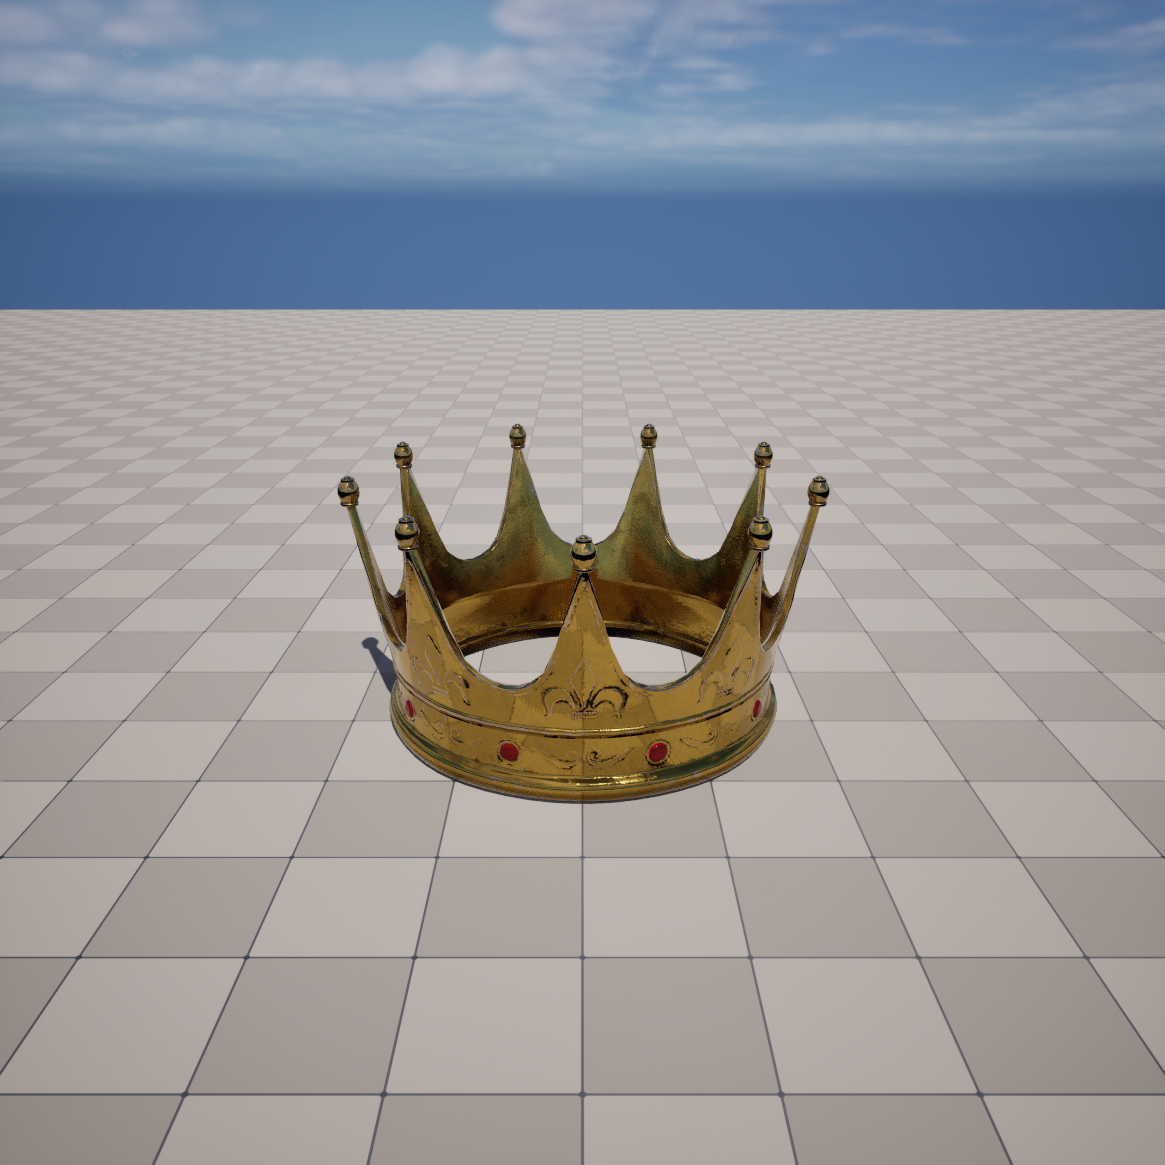
\includegraphics[width=\linewidth]{asset_error/right_crown.png}
    \caption{数字资产皇冠的渲染结果}
  \end{subfigure}
  \begin{subfigure}[t]{0.45\textwidth}
    \centering
    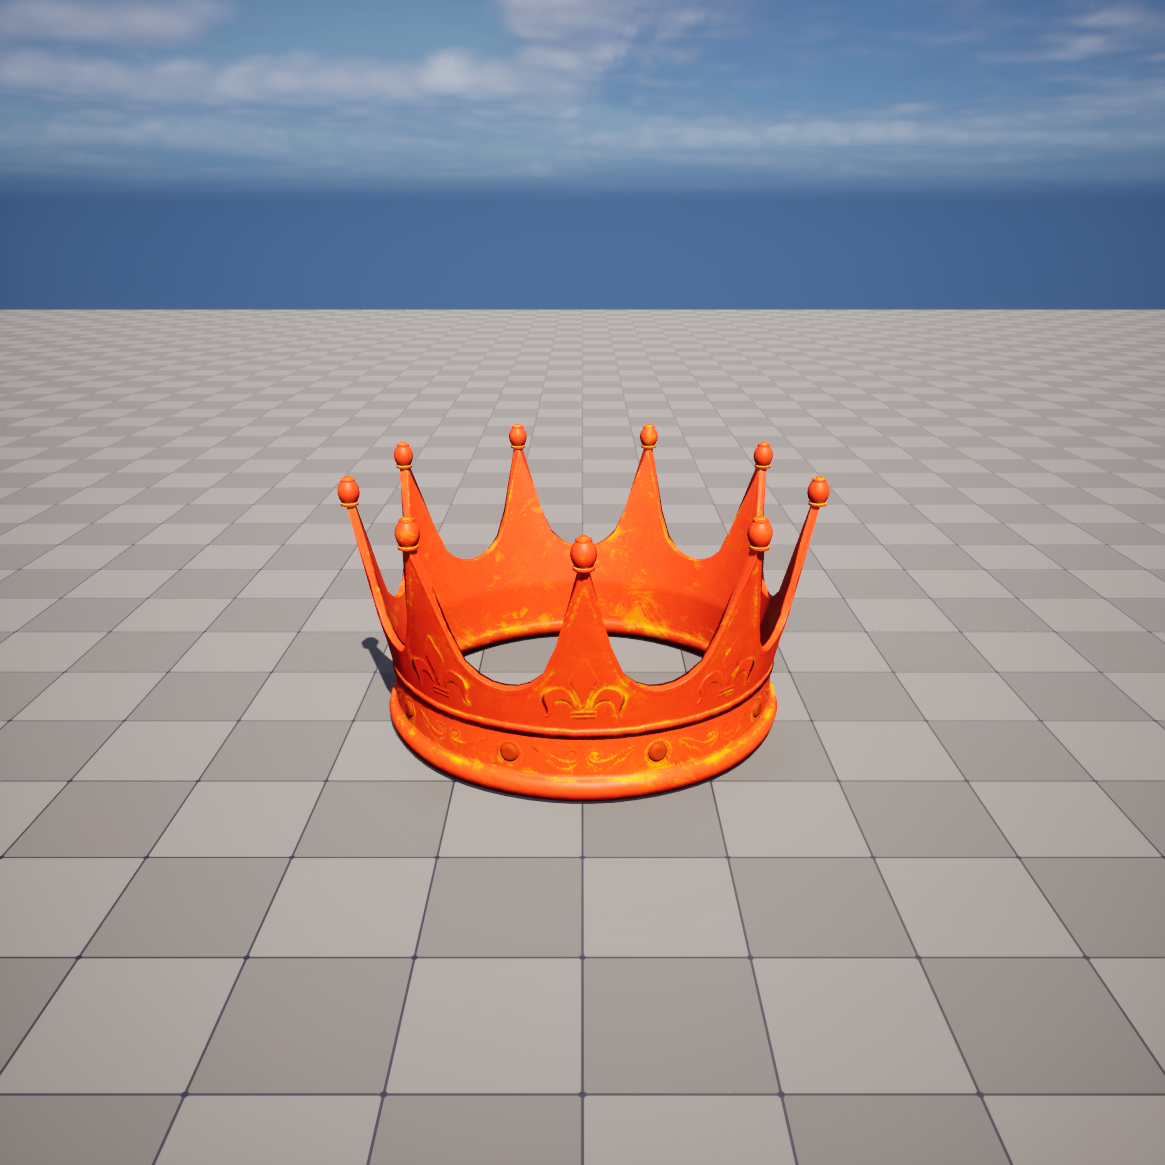
\includegraphics[width=\linewidth]{asset_error/wrong_crown.png}
    \caption{渲染技术不匹配时的错误结果}
  \end{subfigure}
  \caption{数字资产及渲染}
  \label{fig:asset_rendering}
\end{figure}
\subsection{研究意义}
为了尽可能减少二者耦合带来的负面影响,
在传统渲染管线中,不同领域和应用场景往往形成了各自的工作流(Workflow),
这些工作流根据不同的渲染技术设计了不同的资产制作规范和后续编辑流程。
在实际开发时,资产只需严格遵循工作流的相应标准进行制作,即可保证有相应的渲染技术能够对其渲染。

近年来,深度学习技术在计算机图形学领域崭露头角,
其中神经辐射场(Neural Radiance Fields,NeRF)作为一种新兴的三维场景表示方法,
通过隐式地将场景编码为连续的辐射场和体积密度场,实现了从稀疏二维图像重建三维场景的突破。
NeRF无需依赖显式的网格、点云或体素数据,从而避免了离散表示带来的伪影和内存开销,
展现了极高的通用性和灵活性。因此,本文旨在通过NeRF这种新颖的场景重建与表示技术,
解决数字资产与渲染技术之间紧密耦合的问题。本文提出了一套创新的NeRF光照分解管线。
该管线通过结合NeRF和可微渲染技术,首先从二维图像中建立场景信息,
随后将场景信息分解为显式的几何形状与反射属性,最终针对特定工作流生成对应的数字资产。
相对于已有研究,本文的具体改进包括:

\begin{itemize}
  \item 直接输出显式几何表示:采用混合几何表示方法,
  使得管线能够直接输出可编辑的网格模型。
  因此,我们管线生成的几何形状可以无缝对接传统渲染器,并用于后续编辑任务。
  \item 工作流驱动的反射属性解耦:通过将纹理以多层感知机的形式表示,
  灵活地描述了场景表面反射属性与特定工作流之间的映射关系,
  从而实现资产在不同工作流之间的转换,降低数字资产制作的严格性和开发成本。
  \item 阴影感知的神经光照:设计了神经光照表示,
  通过对直接光照、阴影和环境光照的合理分解与建模,
  提高了管线在复杂光照条件下的表现,使得输出结果更符合实际物理规律。
\end{itemize}

综上所述,本课题旨在通过构建基于NeRF和可微渲染的光照分解管线,
打破传统渲染技术与数字资产之间的紧密耦合关系,
为多种渲染工作流提供一种灵活、可编辑的数字资产表示方案。
本文的方法能够使得旧有资产不因技术不兼容被废弃,节省大量人力成本。
同时,也能允许开发者和创作者可以根据项目需求灵活切换工作流,提升创作自由度,
从而推动数字内容生产与渲染技术的发展。



\section{国内外研究现状}
\subsection{用于表征三维场景的神经辐射场}
NeRF利用神经网络来表示三维场景,并通过多层感知机器(Multilayer Perceptron,MLP)或其他网络参数生成新视角图像,
这一方法近年来受到广泛关注。传统方法[1–5]通常采用显式的离散表示来构建三维场景,
但显式离散表示在利用梯度优化网格几何和拓扑结构时存在较大局限性,
因此研究者们逐渐转向基于连续体积的表示方案。

Mildenhall等人[6]提出了可微分体积渲染技术,用密度$\sigma$来描述体积,
通过光线步进在五维辐射场中计算出射辐射,从而实现图像渲染。
尽管这种方法在新视角合成上取得了令人印象深刻的成果,但由于体积渲染的固有局限,
所生成的几何细节往往会显得模糊,无法还原高频细节。

为了解决这一问题,后续研究主要集中在两个方向:一是探索改进的网络结构以保留更多场景细节[7–10];
二是在不牺牲视觉质量的前提下,优化神经辐射场的训练与推理速度[11,12]。
同时,也有部分研究尝试采用基于表面的渲染方法,直接对物体表面进行优化。
例如,NeuS[13]通过有向距离函数(Sign Distance Function,SDF)来表示形状,
并利用从SDF到密度的无偏转换,使得该方法能够兼容NeRF的渲染框架。

然而,由于以上这些方法将场景信息编码为辐射场,场景中的每一个着色点均被视为自发光光源,
因此以上方法均依赖于体积渲染和光线步进来生成图像。相较于传统渲染,体积渲染的计算开销更大,
并且在光照等方面需要采用近似计算,这在一定程度上影响了着色模型的表现能力。
其次,这种编码方式使得NeRF易于完成新视角合成任务,
但限制了NeRF在下游编辑任务中的应用,也难以直接嵌入传统渲染引擎中。


\subsection{神经辐射场的光照分解}

为了弥补上一节中所述的这些不足,近期研究[14–16]尝试将NeRF与可微渲染技术相结合,在同一管线下联合优化,
从而将场景信息分解为几何形状和反射属性,以便在新的光照条件下实现重渲染或进一步编辑。
可微渲染旨在从观测图像中分离出物体的几何结构、材质属性和光照条件,将可微渲染融入NeRF框架的方案通常称为NeRF光照分解管线,
其研究重点在于如何准确地表示场景中的几何形状、反射属性和光照,以及如何选择合适的着色模型进行渲染。
下面将依次介绍现有方法在各个方面的研究现状。

\fourthtitle{1}反射属性表示

反射属性描述了光线在物体表面反射的特性。由于可微渲染为高度不适定(Highly ill-posed)的问题,
比如着色点颜色较亮既可能是由于粗糙浅色表面的漫反射产生,也可能是因为光滑深色表面的镜面反射导致,
因此先前的工作[27,28]中通常旨在恢复兰伯特(Lambertian)表面,即忽略掉高光反射属性。
近期工作中多使用基于物理的着色模型,其使用双向反射分布函数(Bidirectional reflectance distribution function,BRDF)[29] 来定义从反射属性到光照反射方式的计算过程。NeRFactor[18]采用了数据驱动的BRDF,即将BRDF整体作为一个输出函数直接估计,从而省略了将反射属性转换为BRDF的过程以降低误差。Nerf2Mesh[30]则使用了近似的着色模型,抛弃了反射属性的物理意义,其管线的输出仅能使用特定的着色器。这种方式虽然在一定程度上简化了问题,但导致输出的BRDF缺乏直观的物理意义,比如在传统渲染引擎中,多采用参数化BRDF(如Disney Principled BRDF[31])使得材质编辑更加直观。
另外,由于基于物理的着色模型在真实感上的优越性能,所有的研究均采用了其或其近似。
但本文的目标旨在实现数字资产与渲染技术之间的解耦,数字资产可能需要多种着色模型进行渲染,
因此有必要对其进行扩展。为解决这些问题,本文提出的管线可以自定义不同的着色模型,
并通过材质管理的方式进行组织,以对应不同的工作流。这不仅使得输出结果能够直接用于传统渲染和后续编辑,
同时也实现了基于指定工作流的反射属性进行可微渲染的功能。

\fourthtitle{2}几何形状表示

几何形状表示的目标在于准确描述物体的空间结构和形态,为后续渲染与编辑奠定基础。
目前,大多数工作采用隐式神经表示来捕捉几何信息。虽然隐式神经表示在新视角合成任务中表现出色,
但其通常难以直接获得高质量的显式几何结构。其中,NeRD[17]维持了大部分原有的NeRF管线,
并且直接使用密度体积来表示几何形状。NeRFactor[18]在原有NeRF框架的基础上,
利用NeRF中的粗采样网络提取出神经表面,并在表面上进行后续的渲染步骤。
而其余大部分工作则根据NeuS[13]对NeRF的改进,使用SDF来表示几何形状,旨在还原更多高频细节,
如NeILF++[19]、PhySG[20]、NeRO[21]。然而这些工作使用的均为隐式神经表示,
主要面向重照明任务设计,而未专门针对下游编辑及传统渲染器渲染而优化。
针对这一局限,本文在NeRF光照分解任务中提出了一种基于混合几何表示方法的辐射场分解管线。
该方法能够将任意场景下的辐射场分解为显式表示的网格体,从而直接支持下游编辑任务与传统渲染技术。

\fourthtitle{3}光照表示

光照表示旨在描述场景中的光源分布、照明环境以及光与物体相互作用的方式,
是实现真实渲染的关键环节。NeRF2Mesh[21]认为复杂的着色过程会折损管线的几何重建效果,
因此不使用独立建模的光照表示。大多数现有方法对全局照明做出近似建模,
例如利用球面高斯(Spherical Gaussians,SGs)[17,20]、球面谐波(Spherical Harmonics,SHs)[24]、
低分辨率环境图点光照[18]。部分方法[25]虽尝试结合蒙特卡洛方法(Monte-Carlo Method,MC),
但往往仅捕捉直接照明或要求预先知晓光照环境[26],而其余大部分工作则未能有效处理阴影与可见性问题。
为了解决可微渲染中的光照无法高效表示阴影的问题,本文创新性地设计了一种基于条件输入的阴影调制模块,
能够将直接光照和环境光照根据阴影进行结合,并利用一个预训练的自动编码器定义了物理真实感和平滑的潜空间,
在不需要过高的额外计算成本的前提下提高了光照表示技术对阴影的处理能力。

\subsection{本文的主要贡献与创新}

本文设计的光照分解管线共为两个阶段,分别是利用NeRF建立神经辐射场,随后使用可微渲染分解神经辐射场,
最终获得指定标准的数字资产。本文的创新集中在1.2.2节所述的三个部分。针对光照表示,
本文设计了一种基于条件输入的阴影调制模块,并将其用于阴影感知的神经光照(Shadow-Aware Neural Light, SaNL),
创新地将直接光照和环境光照之间的关系融入其中,提升了光照方法的表示能力。在反射属性表示方面,
本文的管线允许选择自定义的着色模型,并且将反射属性和着色模型表示为MLP材质,
赋予了管线输出任意工作流对应的数字资产的能力。最后,在几何形状表示方面,本文采用显式和隐式混合的表示方法,
解决了现有研究仅能将结果用于重光照和新视角合成的问题,实现了管线输出结果能够直接用于传统渲染和下游编辑。

总的来说,本文的贡献可以总结为:

\begin{itemize}
  \item 本文设计并实现了基于NeRF的资产解耦管线,以神经隐式表示存储数字资产,并以指定标准的工作流降维分解。
  该管线借助NeRF和可微渲染,解决了传统管线导致的数字资产与渲染技术之间的耦合,能够大幅节省游戏、影视等行业中的开发成本。
  \item 本文提出了阴影感知的神经光照表示SaNL,并使用即时渲染引擎和大量环境光照生成了阴影-光照数据集,
  训练了带有阴影关系、物理真实感和连续性等先验知识的神经环境光照。实验表明,使用SaNL后管线的分解效果优于现有的光照表示方式。
  \item 本文在管线中引入DMTet,实现了隐式和显式混合的几何形状表示方式,
  并设计了与其相匹配的损失函数以提高几何形状的分解效果。结合传统的纹理处理技术,
  本文的管线可以直接输出显式网格体表示的数字资产,无缝衔接了分解管线到传统的渲染任务或下游编辑。
\end{itemize}

\subsection{本文结构安排}
本小节将介绍论文结构安排概括,包含每一章节的主要内容和研究重点,以清晰地向读者展示本文研究路线和学术价值。

第二章,相关技术基础。在第二章中,本文将详细介绍本文研究内容的理论基础。为了理解神经辐射场,本文首先解释介绍深度学习的基本概念。然后,本文将深入讲解神经辐射场的理论基础,并阐述其前沿研究进展。最后,本文将讨论神经辐射场分解与可微渲染的理论基础,为后续章节中进一步讲解本文研究内容提供必要的理论支撑。

第四章,阴影感知的光照表示研究。第四章将介绍本文设计的用于表示光照的神经网络,由于本文在第三章中观察到管线对阴影中的场景还原不加,因此创新性地设计了一种神经光照表示以解决该问题。第四章从设计动机以及选用的基础结构出发,讲解本文创新性的阴影光照先验,并通过多个维度对该网络进行实验评估,以验证其有效性。

第三章,数字资产解耦管线的实现。第三章将介绍本文对数字资产解耦管线这一目标的具体实现。首先本文通过混合的几何表示方式解决了现有分解管线无法将输出直接用于传统渲染器的问题,并设计了一种创新的训练策略提高了几何形状建立的准确度。同时,本文为了更好地满足多种工作流的解耦,引入了基于MLP的纹理来表示反射属性。最终本文实现了对数字资产解耦这一目标,并完成了神经辐射场到传统上下游任务的无缝衔接。本文通过实验进一步证明了本文提出方法的可靠性和实用性。

第五章,总结与展望。本章总结了本课题的研究内容和研究成果,讨论了研究中的创新与不足,以及本课题未来可能的改进方向和研究路线。

